
%%%%%%%%%%%%%%%%%%%%%%% file typeinst.tex %%%%%%%%%%%%%%%%%%%%%%%%%
%
% This is the LaTeX source for the instructions to authors using
% the LaTeX document class 'llncs.cls' for contributions to
% the Lecture Notes in Computer Sciences series.
% http://www.springer.com/lncs       Springer Heidelberg 2006/05/04
%
% It may be used as a template for your own input - copy it
% to a new file with a new name and use it as the basis
% for your article.
%
% NB: the document class 'llncs' has its own and detailed documentation, see
% ftp://ftp.springer.de/data/pubftp/pub/tex/latex/llncs/latex2e/llncsdoc.pdf
%
%%%%%%%%%%%%%%%%%%%%%%%%%%%%%%%%%%%%%%%%%%%%%%%%%%%%%%%%%%%%%%%%%%%


\documentclass[runningheads,letterpaper]{llncs}

\usepackage{amssymb}
\setcounter{tocdepth}{3}
\usepackage{graphicx}
\usepackage[]{epstopdf}
\usepackage{amsmath}
\usepackage{url}
\newcommand{\keywords}[1]{\par\addvspace\baselineskip
\noindent\keywordname\enspace\ignorespaces#1}

\begin{document}

\mainmatter  % start of an individual contribution

% first the title is needed
\title{\LARGE{Report for CS 6751, Spring 2017} \\ \Large{Grasping and Prehensile Manipulation Project}}

% a short form should be given in case it is too long for the running head
\titlerunning{Report for CS 6751, Spring 2017}

% the name(s) of the author(s) follow(s) next
%
% NB: Chinese authors should write their first names(s) in front of
% their surnames. This ensures that the names appear correctly in
% the running heads and the author index.
%
\author{Vighnesh Vatsal}
%\thanks{Please note that the LNCS Editorial assumes that all authors have used
%the western naming convention, with given names preceding surnames. This determines
%the structure of the names in the running heads and the author index.}%
%\and Ursula Barth\and Ingrid Haas\and Frank Holzwarth\and\\
%Anna Kramer\and Leonie Kunz\and Christine Rei\ss\and\\
%Nicole Sator\and Erika Siebert-Cole\and Peter Stra\ss er}
%
\authorrunning{Vighnesh Vatsal}
% (feature abused for this document to repeat the title also on left hand pages)

% the affiliations are given next; don't give your e-mail address
% unless you accept that it will be published
\institute{Sibley School of Mechanical and Aerospace Engineering\\
Cornell University}
%Tiergartenstr. 17, 69121 Heidelberg, Germany\\
%\mailsa\\
%\mailsb\\
%\mailsc\\
%\url{http://www.springer.com/lncs}}

%
% NB: a more complex sample for affiliations and the mapping to the
% corresponding authors can be found in the file "llncs.dem"
% (search for the string "\mainmatter" where a contribution starts).
% "llncs.dem" accompanies the document class "llncs.cls".
%

%\toctitle{Lecture Notes in Computer Science}
%\tocauthor{Authors' Instructions}
\maketitle


%\begin{abstract}
%The abstract should summarize the contents of the paper and should
%contain at least 70 and at most 150 words. It should be written using the
%\emph{abstract} environment.
%\keywords{We would like to encourage you to list your keywords within
%the abstract section}
%\end{abstract}

%\section{Introduction}

\section{Introduction} \label{sec:intro}
Grasping end-effectors are one of the most commonly employed manipulation tools in robotic arms. This has followed historically from designs of anthropomorphic end-effectors that mimic the grasping motion performed by the human thumb and forefingers. While grasping is indeed an important function of our hands, it is far from the only mode of interaction between our hands and the environment.

Grasping an object in one's hand effectively turns it into an extension of the arm, being completely constrained and moving with the human arm. However, there are numerous scenarios where such a constraint is neither desired nor necessary. For example, if the task at hand is to move a large block of wood over a flat surface, it would be impractical to try and grasp it. Instead, most people would try to push it along the surface. Another mode of interaction is \textit{caging}, where the body is free to move within the gripper but cannot escape it. An example of this mode would be sliding a mug along a table while it is loosely held within the hand. As humans, we also use a host of other factors to arrive at a manipulation mode, such as gravity, friction, the shape, size and weight of the object, and implicitly, the shape, size and effort capabilities of our own hands.  

However, when imbuing robots with manipulation capabilities, the focus has not been on these less-constrained modes. The reasons for this range from safety to computational planning load. Expending extra effort to tackle uncertainties in the pose of an object being manipulated by a robot using a less-constrained mode was not desirable. The planning problem for a robotic arm remains virtually unchanged if the object is simply added as a rigid body at the end of the kinematic chain. Therefore, most state of the art robots and manipulation planners treat the problem as being divided into two parts: finding a grasping pose, and then performing a motion with the object firmly grasped. This approach is fairly efficient and useful in multiple real-world applications. However, by ignoring the possibility of other modes of manipulation, robots are unable to perform a range of tasks that humans are capable of. As another consequence of this single-minded focus on grasping, we encounter robot motions that seem highly non-intuitive and inefficient to a human observer.       

I aim to extend the state of the art by generating a planner that can switch between pushing, caging and grasping based on the environment and goal for a particular prismatic object. At present, an approach based on tree-search is being explored where the switching condition emerges as a consequence of a suitable search heuristic cost function. This approach is being implemented on a Baxter commercial robot with two-fingered grippers as the end-effectors of two 7-DoF arms.

\section{Literature Review} \label{sec:lit_review}
Most literature on grasping-based manipulation~\cite{prattichizzo2016grasping} considers the scenario in which the robotic arm firmly grips the object, immobilizing it and making it a part of the arm. To place the object in its desired goal configuration is then considered to be a path-planning problem in the $C$--space of the robotic arm~\cite{brock2008motion}, which has been augmented with the grasped object. 

On the contrary, humans tend not to manipulate objects in their environment with only pick-and-place style grasping. For instance, to move a box across a table, one may slide it over the surface by pushing~\cite{chavan2015prehensile}. This form of motion is termed as \textit{prehensile} manipulation. In this class of motion, the object is not assumed to be an extension of the manipulator. Based on the geometry of the object and the robot's end-effector, we can identify configurations that either completely immobilize an object (grasps), or constrain it in such a way that it cannot escape to infinity, but is not completely immobilized (cages). The full geometric framework for these conditions is presented in~\cite{rodriguez2012caging}.

Broadly, we can distinguish between control and planning for manipulation tasks. Planning methods take the full plan of action into account, generally simulating the whole process offline to check for conditions of feasibility and optimality~\cite{kavraki2016motion} of the motion. Control-oriented approaches tend to be real-time, sensor feedback-based methods that aid in the performance of the motion at an implementation level~\cite{dafle2014extrinsic}, generally ensuring local optimality. Task Frame representational approaches~\cite{prats2010framework}, and methods involving friction and physics modeling~\cite{chavan2015prehensile} tend to fall into this category.

This project is aimed at developing a manipulation planner for a robot arm that uses the motion primitives of grasping, caging, and pushing, along with arm translation and rotation. Thus far, most prior work on planning has assumed the grasping primitive to be true, thus reducing the problem to finding a path in $C$--space of the robot. One such set of algorithms distinguishes between \textit{transit} paths, where the object is not in contact with the robot, and \textit{transfer} paths, where the contact is achieved~\cite{alami1994two}. In the interim of switching between these two modes, it is assumed that an immobilizing grasp can be found. Work specific to prehensile motions (caging, pushing) includes efforts to geometrically model a pushing motion to facilitate a grasp~\cite{dogar2010push}, and caging-specific tree-search based algorithms~\cite{diankov2008manipulation}. There have also been efforts to incorporate object physics, friction and mechanics modeling for highly dynamic motion plans that allow for the object to move as an independent object during the plan~\cite{dogar2012physics}. Finally, there are task-space based planners that assume a quasi-static motion of objects, while taking into account the uncertainty in their position, implemented using an RRT-based search~\cite{berenson2009addressing}.




\section{Technical Description}

\subsection{Motion Primitives}
\begin{figure}
\centering
	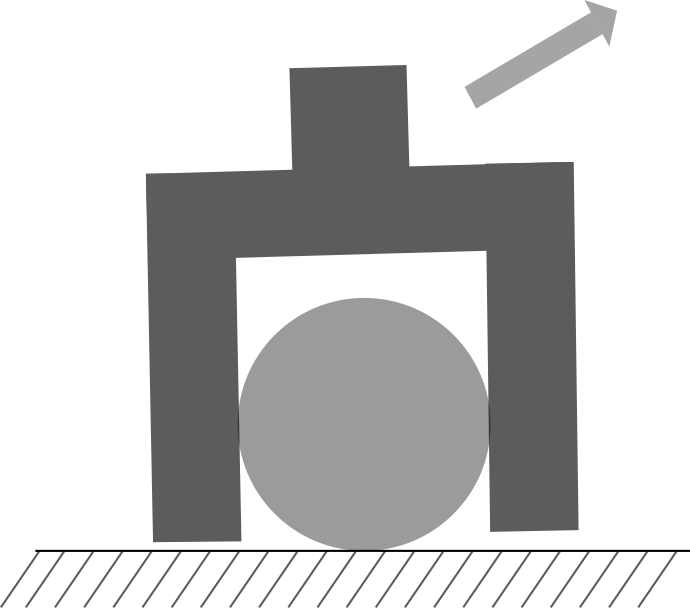
\includegraphics[height=0.2\columnwidth]{images/grasping.png}
 	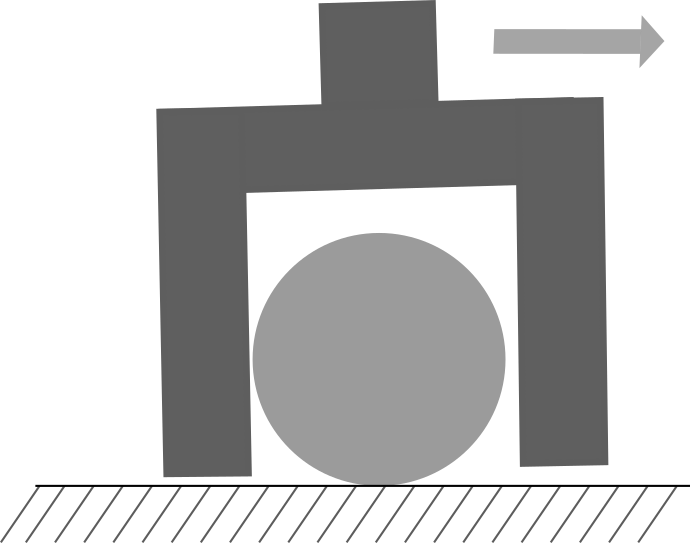
\includegraphics[height=0.2\columnwidth]{images/caging.png}
	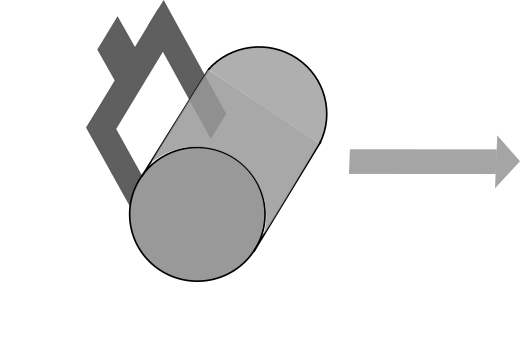
\includegraphics[height=0.2\columnwidth]{images/pushing.png}
\caption{The three motion primitives in the manipulation task with a two-finger gripper and a pipe: grasping, caging, and pushing}
\label{fig:primitives}
\end{figure}

The manipulation task to be performed in this work is for a two-finger end effector-based robotic arm to take an object from an initial state to a specified goal state. To accomplish this, the robot makes use of three manipulation primitives (Fig.~\ref{fig:primitives}):
\begin{itemize}

\item \textit{Grasping:} As mentioned in Section~\ref{sec:lit_review}, this is the most commonly employed manipulation primitive in robotic arms. It involves a full force closure on the object, rendering it immobile and effectively converting it into an extension of the end-effector. It allows for the full 6-degrees of freedom (DoF) translation and rotation of the object.  

\item \textit{Caging:} Caging involves constraining the object such that it is unable to move arbitrarily far away from the end-effector. However, it is free to move within the geometric confines of the end effector. Specifically in the case of a two-finger gripper caging a pipe about its diameter, the pipe is free to move in the axial direction, and free to rotate about any axis. The only constraint is that its center of mass must translate along with the gripper on a flat surface.

\item \textit{Pushing:} Pushing differs from caging in the way that the gripper is unable to rotate the object. It can only slide it along a flat surface while preserving orientation.   
\end{itemize}

\subsection{System Description}
\begin{figure}
\centering
	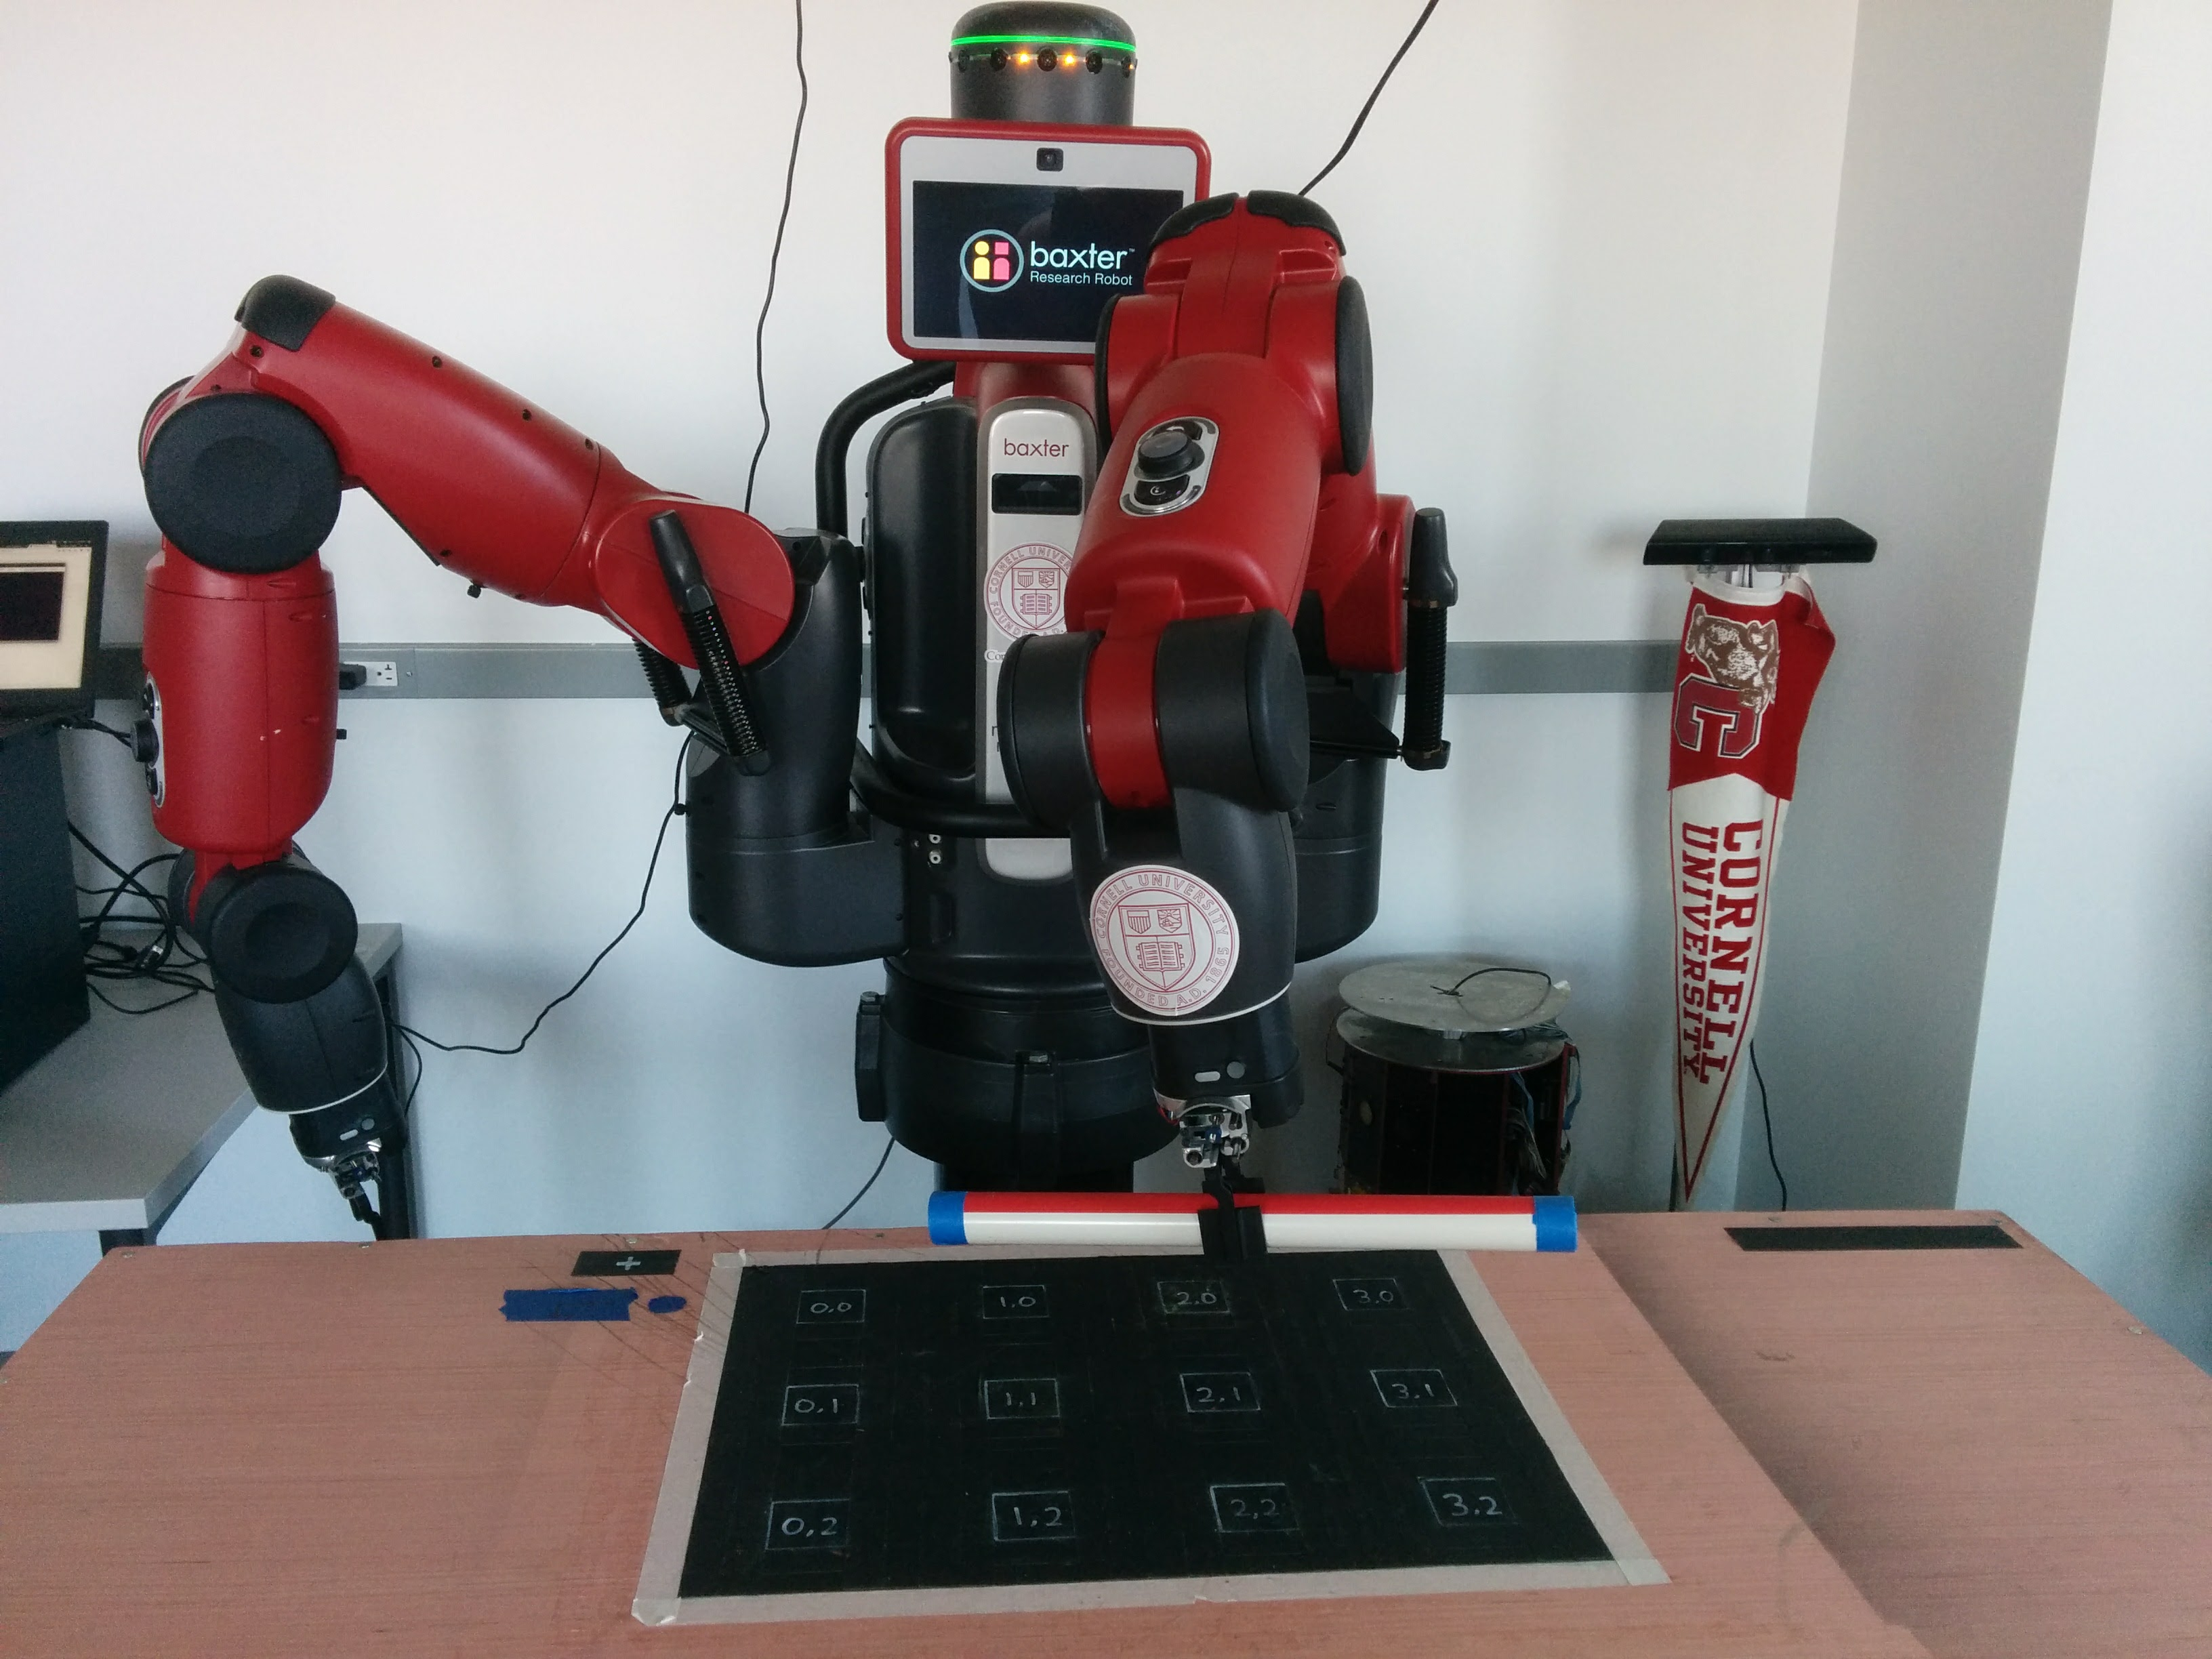
\includegraphics[width=0.9\columnwidth]{images/baxter.jpg}
\caption{Baxter robot system setup for the manipulation task}
\label{fig:system}
\end{figure}

The setup for demonstrating the proposed prehensile manipulation planner consists of the following components: a Baxter robot (Fig.~\ref{fig:system}), an overhead Kinect camera, a flat table, a raised board, and a marked PVC pipe to be manipulated.

There are underlying simplifying assumptions in the structure of this setup:
\begin{itemize}
\item
The PVC pipe is specifically chosen because of its prismatic shape for ease of grasping, pushing and caging it by the Baxter robot's gripper. We are not investigating the effect of object affordances in the present planning scheme. 
\item
All motions are performed in a quasi-static manner. This assumption also implies that there is sufficient friction present between every relevant surface to prevent dynamic motions such as rolling of the pipe while pushing. 
\item
There are no obstacles present in this environment.
\item
The positions the center of mass of every object apart from the pipe are static.
\item
The pipe always remains coplanar with the flat table surfaces. 
\end{itemize}

\subsection{Planning Framework}

\begin{figure}
\centering
	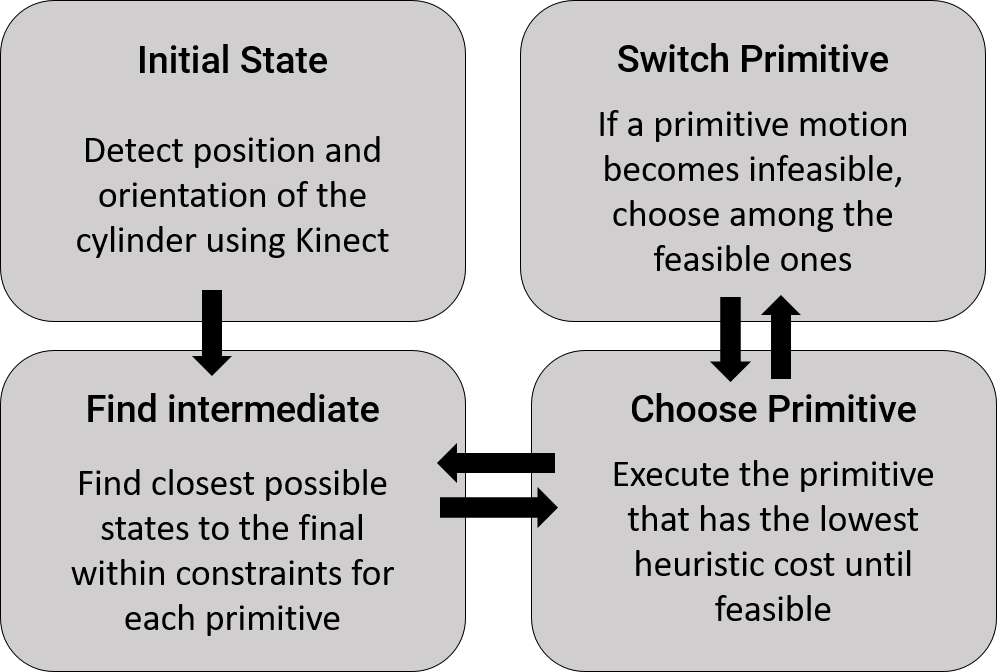
\includegraphics[width=0.8\columnwidth]{images/flow.png}
\caption{Planning framework followed for the manipulation task}
\label{fig:plan}
\end{figure}


The pipe is a rigid body, whose state is $s \in SE(3)$. It can lie on a series of flat planes with fixed $Z$ coordinates and prescribed limits on the $X$ and $Y$ coordinates. The problem statement is then to take the pipe from $s_i \in SE(3)$ to $s_f \in SE(3)$ using a sequence of movements of the robotic arm in its $C$-space. The structure of the problem imposes that only the $(x,y,z)$ and $\theta$ (rotation about the $Z$ axis) coordinates of the pipe are variable. These are computed using RGB-sensing of the end-points of the pipe with a known radius. Since planning is performed in the $C$-space, it is beneficial to formulate the problem in terms of the robot's end-effector. We can use the same four coordinates for this purpose: $(x,y,z,\theta)$, but this time of the end-effector. Each primitive imposes constraints on the motion of the robot end-effector:

\begin{itemize}
\item Pushing requires that $\theta$ and $z$ remain constant, while $x$ and $y$ are variable, normal to $\theta$ of the pipe.
\item Caging requires $z$ to be constant, all other coordinates are variable
\item Grasping imposes no extra constraints
\end{itemize} 

The Open Motion Planning Library (OMPL) allows us to specify initial and final positions for the end-effector in Cartesian space and generates motion plans in the $C$-space for Baxter's arm using the RRT* algorithm. 

Once the initial state of the pipe is known, intermediate states $s_t \in SE(3)$ is found that is as close as possible to $s_f$ within the constraints for each primitive, e.g. if the plan involves pure translation in all three directions, the intermediate state for caging or pushing would be $(x_f,y_f,z_i,\theta_i)$, while that for grasping would be $(x_f,y_f,z_f,\theta_i)$ 

Then for each of these intermediate states, a heuristic cost function $h(p)$ is computed for a path $p$ going from $s_i$ to $s_t$ in the RRT* algorithm:

\begin{equation}
h = f_{energy} + f_{config} + f_{primitive}
\end{equation}\label{eq:heuristic}

Where $f_{energy}$ denotes the energy expended by the robot in performing a plan, $f_{config}$ is the penalty for being far away from the final configuration, and $f_{primitive}$ is the ``ease" of each primitive, following the order pushing $<$ caging $<$ grasping.

The primitive that has the lowest heuristic cost is executed till $s_t$. At this stage, new intermediates are attempted to be found for each primitive. If another primitive has a lower cost, or the others are infeasible, e.g. only grasping can lift the pipe above the table, the planner switches over to another primitive motion, until the goal state $s_f$ is reached.


\section{Implementation}

\subsection{Kinect Sensing and Transformations}

\begin{figure}[ht]
\centering
	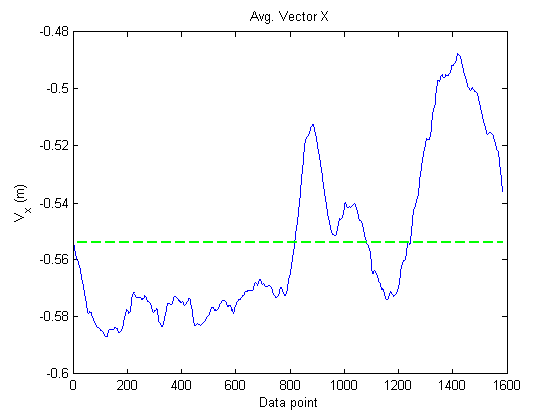
\includegraphics[height=0.3\columnwidth]{images/vec_avg_x.png}
	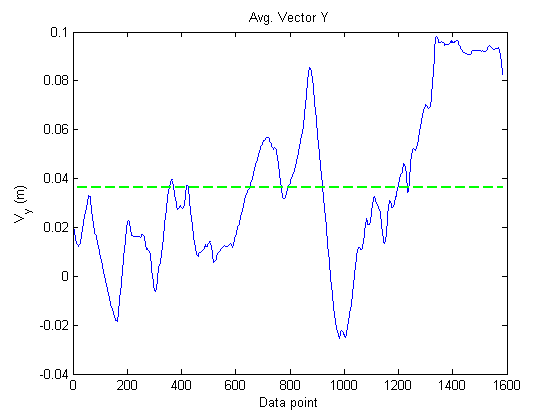
\includegraphics[height=0.3\columnwidth]{images/vec_avg_y.png}
	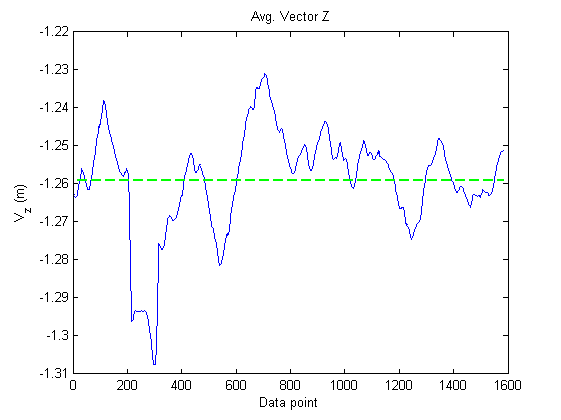
\includegraphics[height=0.3\columnwidth]{images/vec_avg_z.png}
\caption{Components of the position vector between the Kinect and Baxter frames of reference}
\label{fig:kinect_to_baxter}
\end{figure}

The overhead Kinect camera is used to track two colored blocks attached to the end-points of the pipe. All data from the Kinect frame is transformed to the Baxter frame using a homogeneous transformation:

\begin{equation}
\left[ \begin{array}{c} x_{P/B} \\ y_{P/B} \\ z_{P/B} \\ 1 \end{array} \right] = \begin{bmatrix} 0 & 1 & 0 & -x_{B/K} \\ 1 & 0 & 0 & -y_{B/K} \\ 0 & 0 & -1 & -z_{B/K} \\ 0 & 0 & 0 & 1 \\ \end{bmatrix} \left[ \begin{array}{c} x_{P/K} \\ y_{P/K} \\ z_{P/K} \\ 1 \end{array} \right]
\end{equation}

Here $x_{P/B}$ is the position of a point $P$ in the Baxter frame, $x_{P/K}$ is the position sensed in the Kinect frame, and $x_{B/K}$ is the position vector of the Baxter's origin in the Kinect frame.

A calibration routine is performed to find the position vector between the Baxter's origin and the Kinect frame's origin using end-effector position detection built into the robot. The robot's arm is moved through various positions in 3-D such that the end-effector can be tracked by the Kinect sensor. After reducing the signal noise with a moving average filter, the mean value of the position vector is obtained (Fig.~\ref{fig:kinect_to_baxter}).

\begin{figure}[ht]
\centering
	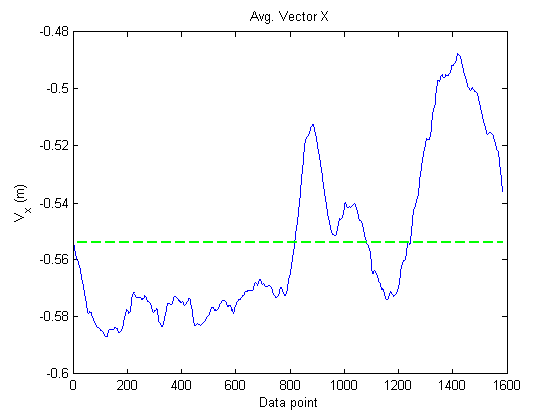
\includegraphics[height=0.3\columnwidth]{images/vec_avg_x.png}
	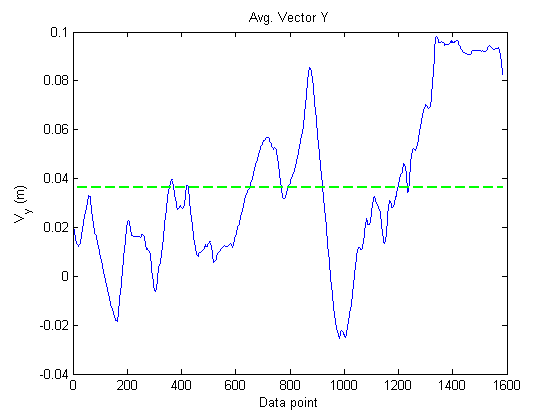
\includegraphics[height=0.3\columnwidth]{images/vec_avg_y.png}	
\caption{Images of the end points of the pipe captured by RGB sensing on the Kinect}
\label{fig:kinect_rgb}
\end{figure}

Once the positions of the end points of the pipe are obtained (Fig.~\ref{fig:kinect_rgb}), its orientation on the table can be determined. This allows us to set a position and orientation of the end-effector appropriately for pushing, caging or grasping. For caging and grasping, the gripper is over the mid-point with the orientation parallel to the pipe's, while for pushing it is at a distance equal to the radius of the pipe away from the mid-point along the normal to the pipe, and oriented along the normal.

\subsection{State Machines: ROS-SMACH}
The planning framework shown in Fig.~\ref{fig:plan} is implemented with state machines using the ROS-SMACH framework. We define the three motion primitive states: pushing, caging and grasping


\subsection{MoveIt! Planning}

\subsection{Results}

\bibliographystyle{splncs03}
\bibliography{IEEEabrv,references}


\end{document}
